\documentclass{article}

%\usepackage{amsthm}
\usepackage{charter}
\usepackage{eulervm}
\usepackage{amsmath}
\usepackage{amssymb}
\usepackage{graphicx}
\usepackage{caption}
\usepackage{subcaption}
\usepackage{enumerate}
\usepackage{cancel}
\usepackage{hyperref}
\usepackage{lscape}

\usepackage{authordate1-4}

\usepackage{color}
\usepackage[usenames,dvipsnames,svgnames,table]{xcolor}

\DeclareMathOperator*{\argmin}{\arg\,\min}
\DeclareMathOperator*{\argmax}{\arg\,\max}

\newcommand{\sdr}[1]{\textcolor{blue}{\small #1\textsuperscript{[sdr]} }}
\newcommand{\pb}[1]{\textcolor{OliveGreen}{\small #1 \textsuperscript{[pb]} }}

\newcommand{\p}{\mbox{\,.}}
\newcommand{\fl}[1]{\left \lfloor #1 \right \rfloor}
\newcommand{\g}[1]{\color{gray} #1 \color{black}}
\newcommand{\hide}[1]{}

\author{Peter Bloem \and Pieter Adriaans}

\title{Empirical survey of complexity measures on graphs, focusing on RDF data and Algorithmic Statistics}
\date{\today} 

% non-indented, spaced paragraphs
\setlength{\parindent}{0.0in}
\setlength{\parskip}{0.1in}


\begin{document}

\maketitle

We have scaled up the results from the previous deliverable in data volume and added various complexity measures. We will process more datasets, and attempt to establish interesting empirical results based on compression and complexity analysis. The existing implementations of complexity measures from 2012Q3 are included as a comparison.

The purpose of this deliverable is threefold. It validates that our methods, such as they are, can be used to provide useful empirical results. It will serve as a test of our software and make sure that it is maintained (preventing `code rust'). Finally, it will provide us with feedback for which features of our code are interesting enough to scale up in quarter 3.

Parts of this document have been taken and adapted from the deliverables of 2012 quarter 2 and quarter 3.

\section*{Code}

The code is written in Java. The JUNG graph library has been replaced with an alternative implemented for the project. All code is available from GitHub in the following repsitory. It is released under an MIT open source license. 
\begin{description}
\item[Lilian] (\url{https://github.com/pbloem/Lilian}) Implementation of the complexity measures, including some tools for running experiments. This repository also contains a great deal of code unrelated to this deliverable. The relevant code resides mostly in the package \texttt{org.lilian.graphs}.
\end{description}

\section{Data}

We test these complexity measures on the following datasets:

\subsection*{Technological networks}

\subsection{An Erdos-Renyi random graph}

A random graph consisting of 1000 nodes, with connection probability 0.5.

\subsection{A preferential attachment random graph}

A random graph consisting of 1000 nodes, generated by the Barabasi Albert algorithm, with 2 connection added per iteration.


\subsubsection*{The internet}

The internet is a classic example of a large, complex graph. So large, in fact that we have little hope of seeing a full snapshot of the whole network at once. The best we can do is to capture some part of it using traceroutes. We use a dataset downloaded from the personal page of Mark Newman (\url{http://www-personal.umich.edu/~mejn/netdata/}), which contains around 23 thousand nodes.

\subsubsection*{Commit social web}

This dataset was produced by the Data2Semantics project to map out the relations within the commit project.

\subsubsection*{IAFB Dataset}

This dataset was included to test our methods on RDF data. We take the dataset from \cite{bloehdorn2007kernel} and disregard any predicates that are not part of the domain specific ontology (http://swrc.ontoware.org/ontology). Named resources, blank nodes and literals are translated to vertices and predicates are translated to edges.

\subsubsection*{The world wide web}

The world wide web, while closely associated with the internet, is a fundamentally different type of network. For example, a link between two systems on the internet will bear some relation to physical proximity of the systems. Linking to a website that is hosted far away costs nothing.

The WWW dataset is know as www-barabasi, and is a common dataset in graph analysis. 

\subsection*{Social networks}
\subsubsection*{Epinions}

Epinions.org is a review site where users can choose to `trust' one another. these trust relations are then used to determine the value of a given review. The total network, downloaded form \url{http://snap.stanford.edu/data/soc-Epinions1.html} contains about 76 thousand nodes.

Originally used in \cite{richardson2003trust}.

\subsubsection*{Pokec relationship network}

Pokec is a Slovakian social networking website. This dataset describes the social relations on the site.

Downloaded from \url{http://snap.stanford.edu/data/soc-pokec.html}. Citations: \cite{takacdata}


\section*{Experiments}

\subsubsection*{Basic complexity measures}

To show the scale of dataset that we can analyse, we perform some basic graph analyses on an datasets of increasing size.

\begin{tabular}{|l | r r r r r r r r |}
  \hline                       
  & $n$ & $l$ & $d_\mu$ & $d_\sigma$ & $W$ & $\omega$ & $\alpha$ & $t$ \\ 
  \hline
er  & $10000$ & $50045$ & $10.009$ & $3.14$ & $10000$ & $0.68$ & $0.0$ & $13.7 s$ \\ 
pa  & $10000$ & $19997$ & $4.0$ & $6.09$ & $10000$ & $0.145$ & $-0.06$ & $11.2 s$ \\ 
internet  & $22963$ & $48436$ & $4.29$ & $32.94$ & $22963$ & $0.030$ & $-0.20$ & $28.7 s$ \\ 
commit  & $18117$ & $56031$ & $6.19$ & $74.83$ & $18117$ & $0.065$ & $-0.13$ & $43.4 s$ \\ 
iafb  & $8318$ & $61255$ & $14.73$ & $69.87$ & $8318$ & $0.13$ & $-0.26$ & $20.6 s$ \\ 
epinions  & $75877$ & $508837$ & $13.41$ & $52.66$ & $75877$ & $0.11$ & $-0.011$ & $15.6 s$ \\ 
barabasi  & $325729$ & $1497135$ & $9.19$ & $48.38$ & $325729$ & $0.050$ & $-0.043$ & $30.0 s$ \\ 
skitter  & $1696415$ & $11095298$ & $13.08$ & $136.86$ & $1694616$ & $0.11$ & $-0.081$ & $7m 36 s$ \\ 
patents  & $6009555$ & $16518948$ & $5.5$ & $9.33$ & $3764117$ & $0.23$ & $0.17$ & $13h 27m 27s$ \\ 
social  & $1632804$ & $30622564$ & $37.51$ & $59.52$ & $1632803$ & $0.49$ & $ 5.3628-4 $ & $33m 34s$ \\ 
  \hline  
\end{tabular}

With the following meanings:
\begin{description}
\item[$n$] The number of nodes in the graph.
\item[$l$] The number of links in the graph.
\item[$d_\mu$] The mean degree.
\item[$d_\sigma$] The standard deviation of the degree distribution.
\item[$W$] The size of the largest weakly connected component.
\item[$\omega$] The wing width ratio \cite{kang2011beyond}.
\item[$\alpha$] The Assortativity
\item[$t$] The total running time of all analyses run for this report. \footnote{note that for graphs with more than 50000 nodes, the AM compressor wasn't run).}
\end{description}

\subsubsection*{Slash-and-burn and spyplots}

We implemented and studied the Slash-and-burn algorithm \cite{kang2011beyond}, and the spyplot method of visualization. This algorithm calculates an order of nodes that is likely to benefit compression (and computation) on real-world graphs.

The following plots show adjacency matrices (spyplots) for the datasets mentioned above.

\begin{table}[h]
\begin{tabular}{l | c c c c}
\hline
 & random & given & degree & sb \\
\hline
er
&
    
\includegraphics[width=0.23\textwidth]{../img/er/adjacency-matrix-random-ordering.png}
& 
    
\includegraphics[width=0.23\textwidth]{../img/er/adjacency-matrix-given-ordering.png}
& 
    
\includegraphics[width=0.23\textwidth]{../img/er/adjacency-matrix-degree-ordering.png}
& 
    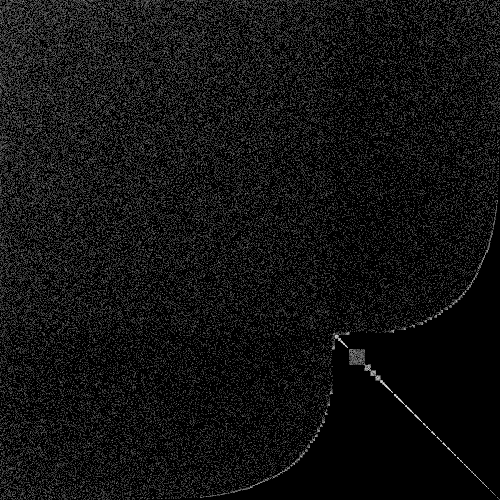
\includegraphics[width=0.23\textwidth]{../img/er/adjacency-matrix-slashburn-ordering.png} \\

\hline
pa
&
    
\includegraphics[width=0.23\textwidth]{../img/pa/adjacency-matrix-random-ordering.png}
& 
    
\includegraphics[width=0.23\textwidth]{../img/pa/adjacency-matrix-given-ordering.png}
& 
    
\includegraphics[width=0.23\textwidth]{../img/pa/adjacency-matrix-degree-ordering.png}
& 
    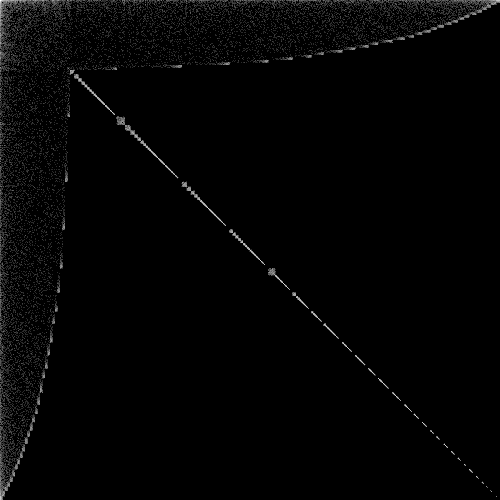
\includegraphics[width=0.23\textwidth]{../img/pa/adjacency-matrix-slashburn-ordering.png} \\

\hline
internet
&
    
\includegraphics[width=0.23\textwidth]{../img/internet/adjacency-matrix-random-ordering.png}
& 
    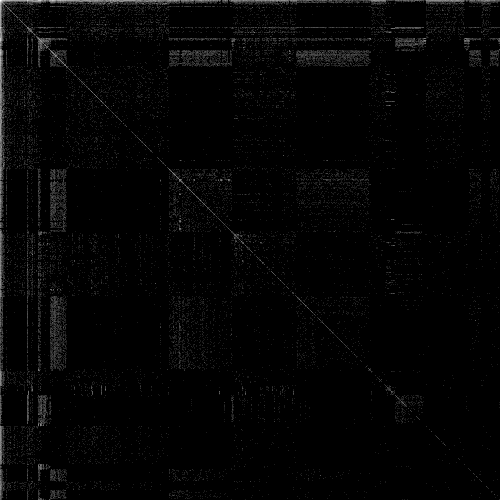
\includegraphics[width=0.23\textwidth]{../img/internet/adjacency-matrix-given-ordering.png}
& 
    
\includegraphics[width=0.23\textwidth]{../img/internet/adjacency-matrix-degree-ordering.png}
& 
    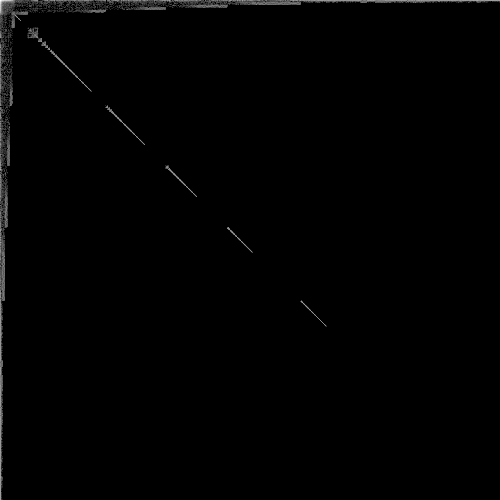
\includegraphics[width=0.23\textwidth]{../img/internet/adjacency-matrix-slashburn-ordering.png} \\

\hline
commit
&
    
\includegraphics[width=0.23\textwidth]{../img/commit/adjacency-matrix-random-ordering.png}
& 
    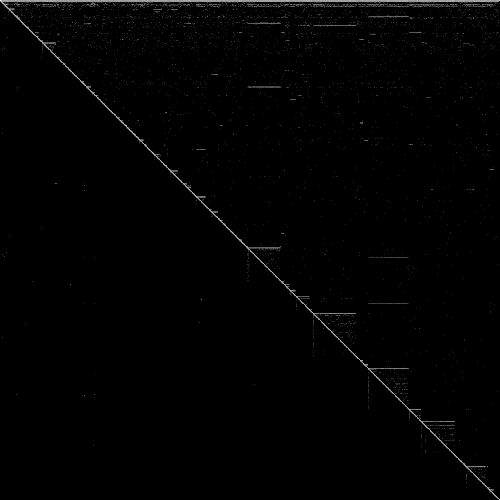
\includegraphics[width=0.23\textwidth]{../img/commit/adjacency-matrix-given-ordering.png}
& 
    
\includegraphics[width=0.23\textwidth]{../img/commit/adjacency-matrix-degree-ordering.png}
& 
    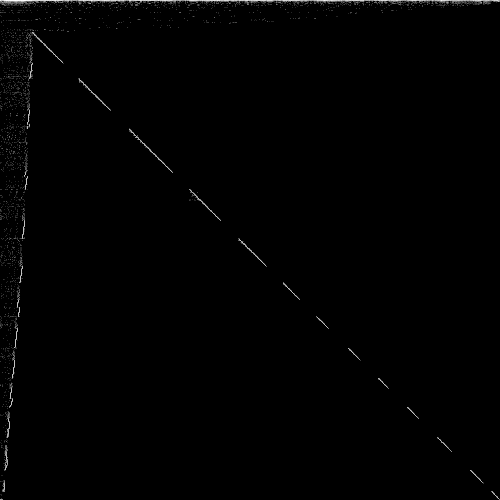
\includegraphics[width=0.23\textwidth]{../img/commit/adjacency-matrix-slashburn-ordering.png} \\

\hline
aifb
&
    
\includegraphics[width=0.23\textwidth]{../img/aifb/adjacency-matrix-random-ordering.png}
& 
    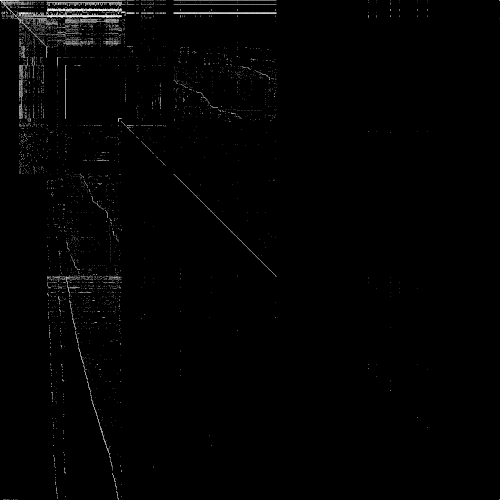
\includegraphics[width=0.23\textwidth]{../img/aifb/adjacency-matrix-given-ordering.png}
& 
    
\includegraphics[width=0.23\textwidth]{../img/aifb/adjacency-matrix-degree-ordering.png}
& 
    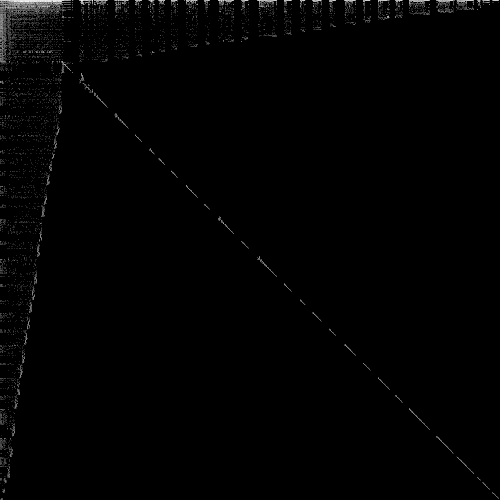
\includegraphics[width=0.23\textwidth]{../img/aifb/adjacency-matrix-slashburn-ordering.png} \\

\hline
epinions
&
    
\includegraphics[width=0.23\textwidth]{../img/epinions/adjacency-matrix-random-ordering.png}
& 
    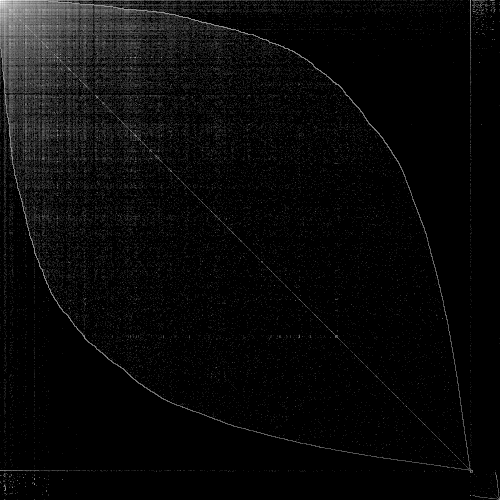
\includegraphics[width=0.23\textwidth]{../img/epinions/adjacency-matrix-given-ordering.png}
& 
    
\includegraphics[width=0.23\textwidth]{../img/epinions/adjacency-matrix-degree-ordering.png}
& 
    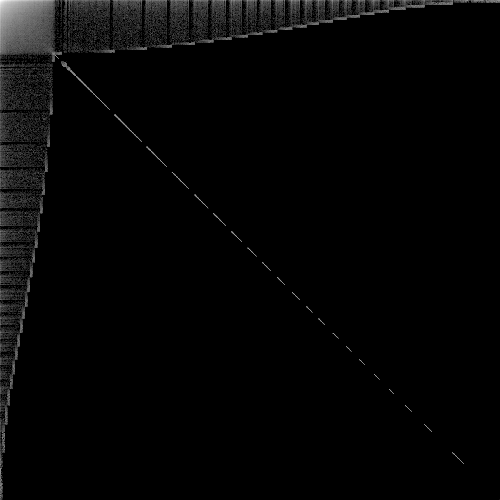
\includegraphics[width=0.23\textwidth]{../img/epinions/adjacency-matrix-slashburn-ordering.png} \\

\hline
barabasi
&
    
\includegraphics[width=0.23\textwidth]{../img/barabasi/adjacency-matrix-random-ordering.png}
& 
    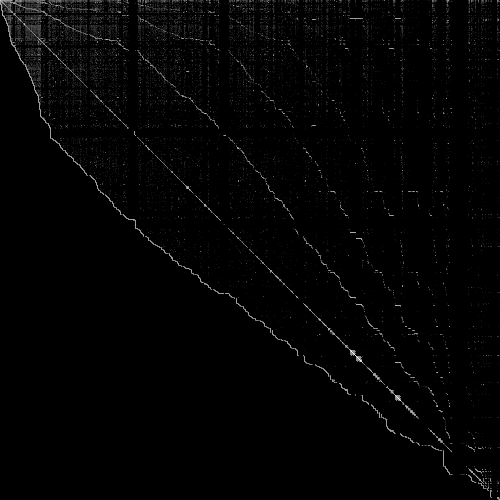
\includegraphics[width=0.23\textwidth]{../img/barabasi/adjacency-matrix-given-ordering.png}
& 
    
\includegraphics[width=0.23\textwidth]{../img/barabasi/adjacency-matrix-degree-ordering.png}
& 
    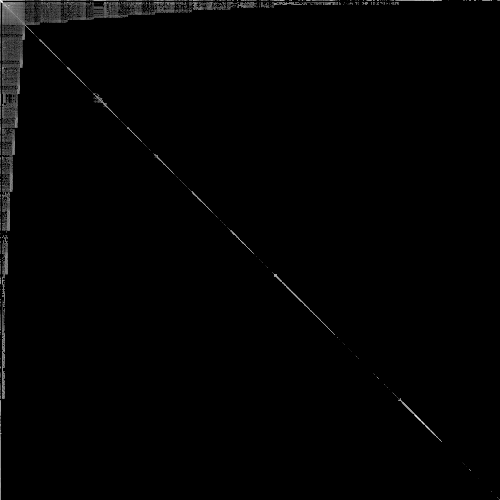
\includegraphics[width=0.23\textwidth]{../img/barabasi/adjacency-matrix-slashburn-ordering.png} \\
    \hline
\end{tabular}
\end{table}

\begin{table}[h]
\begin{tabular}{l | c c c c}
\hline
 & random & given & degree & sb \\
\hline
skitter
&
    
\includegraphics[width=0.23\textwidth]{../img/skitter/adjacency-matrix-random-ordering.png}
& 
    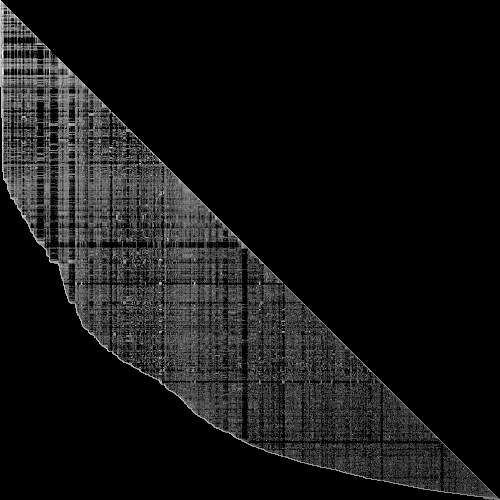
\includegraphics[width=0.23\textwidth]{../img/skitter/adjacency-matrix-given-ordering.png}
& 
    
\includegraphics[width=0.23\textwidth]{../img/skitter/adjacency-matrix-degree-ordering.png}
& 
    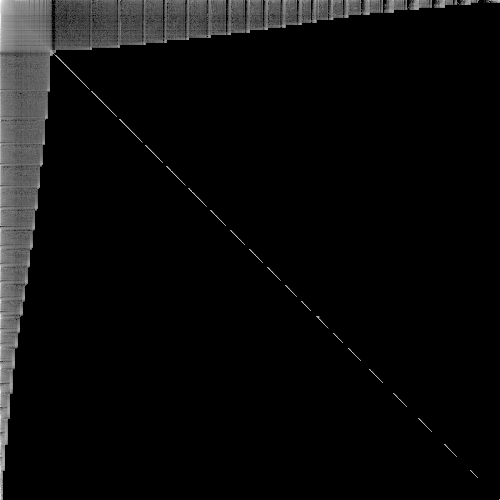
\includegraphics[width=0.23\textwidth]{../img/skitter/adjacency-matrix-slashburn-ordering.png} \\

\hline
patents
&
    
\includegraphics[width=0.23\textwidth]{../img/patents/adjacency-matrix-random-ordering.png}
& 
    
\includegraphics[width=0.23\textwidth]{../img/patents/adjacency-matrix-given-ordering.png}
& 
    
\includegraphics[width=0.23\textwidth]{../img/patents/adjacency-matrix-degree-ordering.png}
& 
    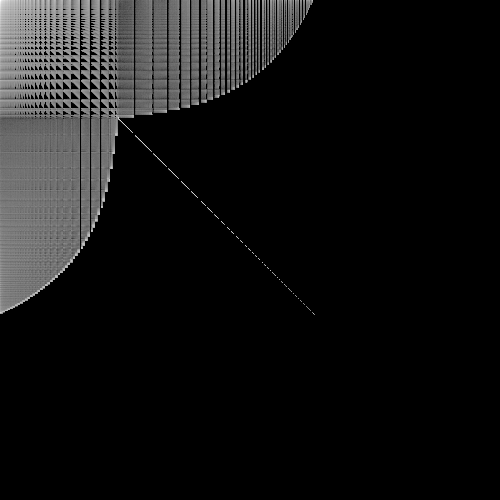
\includegraphics[width=0.23\textwidth]{../img/patents/adjacency-matrix-slashburn-ordering.png} \\

\hline
pokec
&
    
\includegraphics[width=0.23\textwidth]{../img/pokec/adjacency-matrix-random-ordering.png}
& 
    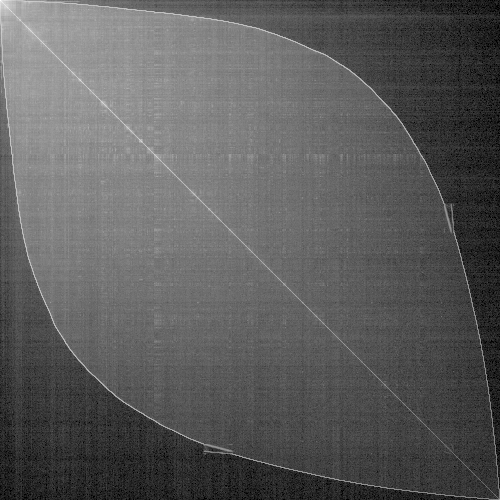
\includegraphics[width=0.23\textwidth]{../img/pokec/adjacency-matrix-given-ordering.png}
& 
    
\includegraphics[width=0.23\textwidth]{../img/pokec/adjacency-matrix-degree-ordering.png}
& 
    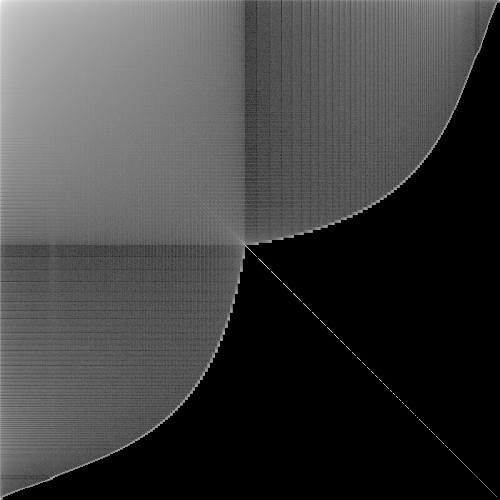
\includegraphics[width=0.23\textwidth]{../img/pokec/adjacency-matrix-slashburn-ordering.png} \\


\hline 

\end{tabular}
\end{table}

\subsubsection*{Compression tests}

Our ultimate goal is to study compression of graphs as a means of performing inference and complexity-analysis.\footnote{See also \cite{bloemcompression}, which was submitted as a deliverable this quarter.} To this end, we study the basic methods of representing graphs in a bitstring, and the effect that node ordsering has on the performance. We test the following methods
\begin{description}
\item[edge list (el)] The graph is stored as a list of prefix-coded pairs of integers representing the graph's edges. 
\item[neighbor list (nl)] The graph is stored as a list of lists of indices. Each list represents the neighbors of a given node. The indices are incremented by one so that the index 0 can be used as a delimiter.
\item[adjacency matrix (am)] We generate an adjacency matrix of $\frac{n^2 + n}{2}$ cells for an undirected graph or $n^2$ cells for a directed graph and flatten this into a bitstring. We zip the resulting string to exploit simple structures within it. We add a single bit to distinguish between directed and underected graphs so that the code is self-delimiting.
\end{description}

\begin{landscape}
\hspace{-1cm}
\begin{tabular}{|l | r r r | r r r | r r r | r r r |}
\hline
\multicolumn{1}{|c}{} & \multicolumn{3}{c}{natural} & \multicolumn{3}{c}{random} & \multicolumn{3}{c}{degree} & \multicolumn{3}{c|}{slashburn} \\
  \hline                       
  & el & nl & am & el & nl & am & el & nl & am & el & nl & am \\ 
  \hline
 er & 1538162 & 816534 & 146338 & 1537724 & 816010 & 146685 & 1494122 & 800123 & 144941 & 1495829 & 801555 & 143144 \\ 
 pa & 558505 & 317266 & 63798 & 615444 & 332357 & 68439 & 546885 & 318000 & 61711 & 551301 & 318136 & 58245 \\
 internet & 1329380 & 808430 & & 1594604 & 860025 & 165759 & 1190776 & 777404 & 114297 & 1224515 & 798488 &  \\
 commit & 1609616 & 673296 &  & 1817950 & 876699 & 215356 & 1370638 & 556954 & 135640 & 1411396 & 558630 &  \\
 aifb & 1583268 & 745875 & 70518 & 1844193 & 927728 & 155225 & 1366585 & 591342 & 69044 & 1403070 & 595136 & 69086 \\
 epinions & 1.5760E7 & 8091701 &  & 1.9181E7 & 9670775 &  & 1.4272E7 & 7530653 &  & 1.4720E7 & 7642574 &  \\
 barabasi & 6.3445E7 & 3.2238E7 & & 6.3769E7 & 3.2175E7 & & 5.0114E7 & 2.5458E7 & & 5.5466E7 & 2.83587E7 & \\
 skitter & 4.84613E8 & 2.2962E8 & & 5.2691E8 & 2.6509E8 &  & 4.2595E8 & 1.8885E8 & & 4.3375E8 & 1.9100E8 &  \\
 patents &  8.8071E8 &  4.5034E8  & & 8.4574E8 & 4.2886E8 &  & 7.6607E8 & 3.8617E8 &  & 7.6810E8 & 3.8725E8 &  \\
 pokec &  1.3859E9 &  6.9489E8  &  & 1.4513E9 & 7.2733E8 & & 1.3180E9 & 6.6017E8 &  & 1.3200E9 & 6.6129E8 &  \\
  \hline  
\end{tabular}
\end{landscape}
\section{Acknowledgements}
This research was supported by the Dutch national program COMMIT.

\bibliographystyle{authordate3}
\bibliography{citations}

\end{document}
